\documentclass[border=20pt,tikz]{standalone}
\usepackage{tikz}
\usetikzlibrary{shapes,arrows,positioning,calc}

\begin{document}

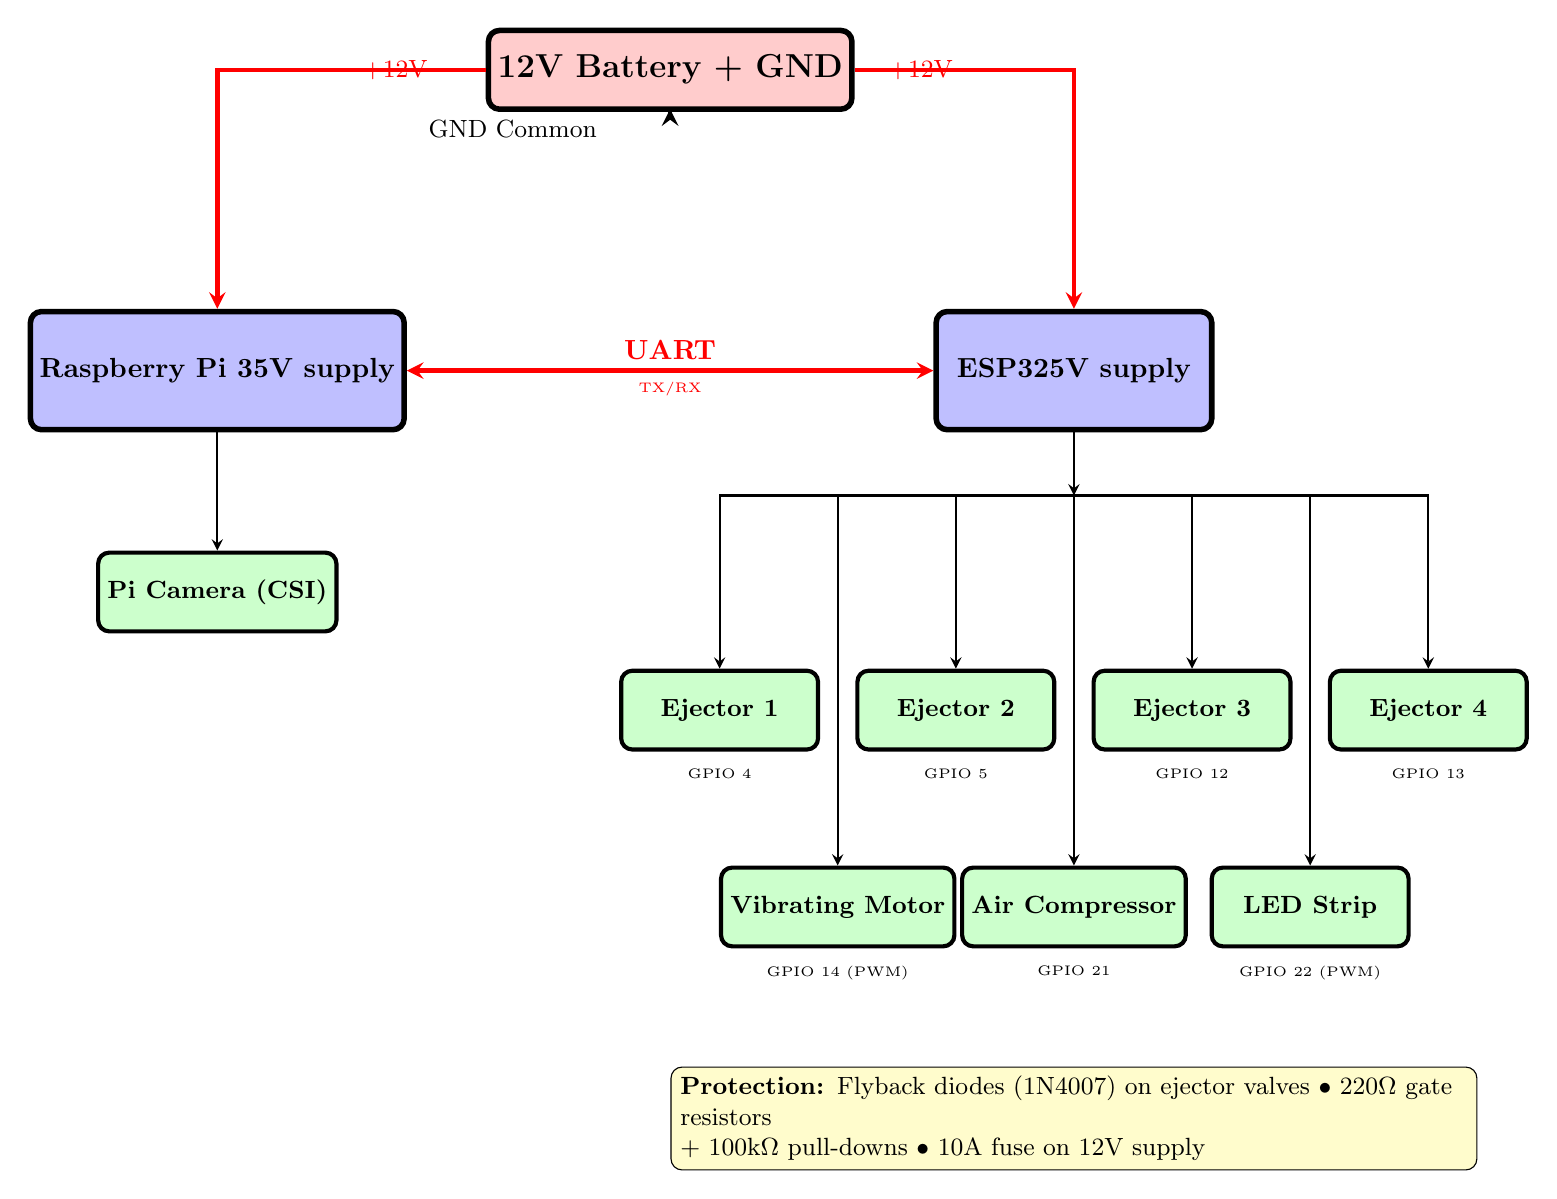
\begin{tikzpicture}[node distance=2.5cm, auto]

% Define styles
\tikzstyle{battery} = [rectangle, rounded corners, minimum width=3cm, minimum height=1cm, text centered, draw=black, fill=red!20, line width=2pt, font=\bfseries\large]
\tikzstyle{processor} = [rectangle, rounded corners, minimum width=3.5cm, minimum height=1.5cm, text centered, draw=black, fill=blue!25, line width=2pt, font=\bfseries]
\tikzstyle{output} = [rectangle, rounded corners, minimum width=2.5cm, minimum height=1cm, text centered, draw=black, fill=green!20, line width=1.5pt, font=\small\bfseries]
\tikzstyle{arrow} = [thick, ->, >=stealth]
\tikzstyle{uart_arrow} = [ultra thick, <->, >=stealth, color=red]

% POWER SUPPLY
\node (battery) [battery] {12V Battery + GND};

% PROCESSORS
\node (pi) [processor, below left=2.5cm and 1cm of battery] {Raspberry Pi 3\\5V supply};
\node (esp) [processor, below right=2.5cm and 1cm of battery] {ESP32\\5V supply};

% Power connections
\draw [arrow, ultra thick, red] (battery) -| node[near start, right] {\small +12V} (pi.north);
\draw [arrow, ultra thick, red] (battery) -| node[near start, left] {\small +12V} (esp.north);
\draw [arrow, ultra thick] (battery) -- ++(0, -0.5) node[below, xshift=-2cm] {\small GND Common};

% UART Communication
\draw [uart_arrow] (pi.east) -- node[above] {\bfseries UART} node[below, font=\tiny] {TX/RX} (esp.west);

% Pi Camera
\node (camera) [output, below=1.5cm of pi] {Pi Camera (CSI)};
\draw [arrow] (pi) -- (camera);

% ESP32 OUTPUTS - Row 1: Ejectors
\node (ej1) [output, below=3cm of esp, xshift=-4.5cm] {Ejector 1};
\node (ej2) [output, below=3cm of esp, xshift=-1.5cm] {Ejector 2};
\node (ej3) [output, below=3cm of esp, xshift=1.5cm] {Ejector 3};
\node (ej4) [output, below=3cm of esp, xshift=4.5cm] {Ejector 4};

% GPIO labels below ejectors
\node [below=0.1cm of ej1, font=\tiny] {GPIO 4};
\node [below=0.1cm of ej2, font=\tiny] {GPIO 5};
\node [below=0.1cm of ej3, font=\tiny] {GPIO 12};
\node [below=0.1cm of ej4, font=\tiny] {GPIO 13};

% ESP32 OUTPUTS - Row 2: Control devices
\node (motor) [output, below=5.5cm of esp, xshift=-3cm] {Vibrating Motor};
\node (compressor) [output, below=5.5cm of esp] {Air Compressor};
\node (led) [output, below=5.5cm of esp, xshift=3cm] {LED Strip};

% GPIO labels below control devices
\node [below=0.1cm of motor, font=\tiny] {GPIO 14 (PWM)};
\node [below=0.1cm of compressor, font=\tiny] {GPIO 21};
\node [below=0.1cm of led, font=\tiny] {GPIO 22 (PWM)};

% Connections from ESP32 to outputs
\coordinate (esp_out) at ($(esp.south) + (0, -0.8)$);
\draw [arrow] (esp) -- (esp_out);
\draw [arrow] (esp_out) -| (ej1);
\draw [arrow] (esp_out) -| (ej2);
\draw [arrow] (esp_out) -| (ej3);
\draw [arrow] (esp_out) -| (ej4);
\draw [arrow] (esp_out) -| (motor);
\draw [arrow] (esp_out) -- (compressor);
\draw [arrow] (esp_out) -| (led);

% Protection note
\node [draw=black, fill=yellow!20, rounded corners, text width=10cm, align=left, below=1.5cm of compressor, font=\small] {
\textbf{Protection:} Flyback diodes (1N4007) on ejector valves $\bullet$ 220$\Omega$ gate resistors \\+ 100k$\Omega$ pull-downs $\bullet$ 10A fuse on 12V supply
};

\end{tikzpicture}

\end{document}
